%==============================================================================
\section{Negative Results: Where DeltaSort Does Not Help}
\label{sec:negative}
%==============================================================================

We document two domains where \DeltaSort does \emph{not} provide a practical
advantage.
Reporting these results is important for delineating the algorithm's useful regime
and preventing over-application.

%------------------------------------------------------------------------------
\subsection{Large-Scale HPC Particle Sorting}
\label{sec:hpc}
%------------------------------------------------------------------------------

\paragraph{Motivation.}
Cosmological N-body and SPH codes (GADGET-4, SPH-EXA) sort particles by
space-filling curve (Morton / Peano-Hilbert) key for cache-efficient neighbor
lookups.
Each timestep, particles move; those crossing a cell boundary constitute
the dirty set $U$.
The integrator already touches every particle, so the dirty set is essentially
free.
This matches the update-aware model.

\paragraph{Setup.}
We simulate $n \in \{10^4, 10^5, 10^6\}$ particles in a 3D box under a leapfrog
integrator.
Morton keys are computed with $\lceil \log_2(n^{1/3}) \rceil$ bits per axis,
giving $\approx n$ cells total (one particle per cell on average).
Three motion regimes control the fraction of cell-crossing particles:

\begin{itemize}
  \item \textbf{Cold:} motion $= 2\%$ of cell width $\Rightarrow k/n \approx 3\%$
  \item \textbf{Warm:} motion $= 10\%$ of cell width $\Rightarrow k/n \approx 16\%$
  \item \textbf{Hot:} motion $= 30\%$ of cell width $\Rightarrow k/n \approx 43\%$
\end{itemize}

Two initial conditions: uniform random (isotropic) and Plummer sphere
(concentrated core).

\paragraph{Results.}

\begin{table}[H]
\centering
\small
\setlength{\tabcolsep}{5pt}
\begin{tabular}{@{}rllrrrr@{}}
\toprule
$n$ & IC & Regime & mean $k/n$ & Full ($\mu$s) & \DeltaSort ($\mu$s) & \ESM ($\mu$s) \\
\midrule
$10^4$  & uniform & cold & 3.3\% & 247 &  36 & 53 \\
$10^4$  & uniform & warm & 15.9\% & 295 & 138 & 105 \\
$10^4$  & uniform & hot  & 42.6\% & 299 & 297 & 219 \\
\midrule
$10^5$  & uniform & cold & 3.4\% & 3380 &  620 & 597 \\
$10^5$  & uniform & warm & 16.0\% & 3639 & 1802 & 1146 \\
$10^5$  & uniform & hot  & 42.7\% & 3825 & 3768 & 2473 \\
\midrule
$10^6$  & uniform & cold & 3.3\% & 44758 & 13603 & 6553 \\
$10^6$  & uniform & warm & 16.0\% & 46318 & 30712 & 13249 \\
$10^6$  & uniform & hot  & 42.7\% & 48611 & 52516 & 29518 \\
\bottomrule
\end{tabular}
\caption{%
  Per-step sort cost in a synthetic HPC simulation.
  \DeltaSort beats the full \texttt{std::sort} baseline by up to $7\times$
  in the cold regime ($n=10^4$), but \ESM is faster than \DeltaSort in most cases.
  At $n=10^6$, \ESM beats \DeltaSort by $1.9\times$ even in the cold regime.
}
\label{tab:hpc}
\end{table}

\paragraph{Finding.}
\DeltaSort outperforms the \texttt{std::sort} (GADGET baseline) by 3--7$\times$
in the cold regime at $n = 10^4$.
However, \ESM consistently outperforms \DeltaSort at $n \geq 10^5$,
even in the cold regime (by 2$\times$ at $n=10^6$).
The reason is cache efficiency: \ESM's linear merge pass is $O(n)$ with excellent
spatial locality, while \DeltaSort's segment scan at large $n$ incurs more
cache misses despite its lower data-movement count.

\paragraph{Verdict.}
For HPC particle sorting at realistic simulation scales ($n \geq 10^5$),
\textbf{\ESM is the better incremental sort, not \DeltaSort}.
\DeltaSort's advantage only materializes at small $n$ ($\leq 10^4$) in the cold
regime---a regime where absolute sort cost is already negligible ($\ll 1\,\mu$s
per particle).
This is an honest negative result: the HPC motivation for \DeltaSort does not
hold at production scale.

%------------------------------------------------------------------------------
\subsection{3D Game Engine Rendering (Bevy)}
\label{sec:bevy}
%------------------------------------------------------------------------------

\paragraph{Motivation.}
GPU-accelerated 3D renderers must sort transparent draw calls by
depth each frame (painter's algorithm).
This is a sort on $n$ \texttt{PhaseItem} structs per frame, with $k$ items
changing depth due to camera or object movement.
In principle this matches the update-aware model; we test whether it matters in practice.

\paragraph{Setup.}
We benchmark Bevy's phase sort using Criterion against two data representations:
\begin{itemize}
  \item \texttt{Vec<PhaseItem>}: contiguous, amenable to \DeltaSort.
  \item \texttt{IndexMap<u64, PhaseItem>}: Bevy's actual production data structure.
\end{itemize}
$n = 100\,000$ draw calls; $k \in \{0, 1, 10, 50, 100, 500, 1000\}$.

\paragraph{Results.}

\begin{table}[H]
\centering
\small
\begin{tabular}{@{}rrrrr@{}}
\toprule
$k$ & Vec full sort ($\mu$s) & Vec \DeltaSort ($\mu$s) & Speedup
    & \% of 16.7\,ms frame \\
\midrule
1   & 215 & 15.8 & $13.7\times$ & 0.09\% \\
10  & 890 & 62.2 & $14.3\times$ & 0.37\% \\
50  & 1956& 150  & $13.0\times$ & 0.90\% \\
100 & 2496& 210  & $11.9\times$ & 1.26\% \\
500 & 3452& 471  & $7.3\times$  & 2.83\% \\
1000& 3289& 702  & $4.7\times$  & 4.21\% \\
\bottomrule
\end{tabular}
\caption{%
  Bevy phase sort: Vec layout, $n=100\,000$.
  \DeltaSort reduces sort latency by 5--14$\times$ but sort remains
  $\leq 5\%$ of a 60\,FPS frame budget for all $k$ tested.
}
\label{tab:bevy-vec}
\end{table}

On the \texttt{IndexMap} (Bevy's actual structure), \DeltaSort beats
\texttt{sort\_by\_key} for $k \leq 10$ ($2.6\times$ speedup) but
\emph{loses} at $k \geq 50$ ($0.86\times$) because recovering dirty indices
from an IndexMap requires a linear scan, eliminating the dirty-set advantage.

\paragraph{Verdict.}
Two independent reasons make 3D rendering a poor target for \DeltaSort:

\begin{enumerate}
  \item \textbf{Budget is too small.} Even without \DeltaSort, a full sort of
    $n=10^5$ draw calls takes $\leq 3.5\,\text{ms}$, which is $<21\%$ of a
    60\,FPS frame (a GPU-bound scene will be bottlenecked on shading long before
    sort matters).
    \DeltaSort reduces this to $\leq 0.7\,\text{ms}$ ($<5\%$), but the savings
    are invisible in end-to-end FPS.
  \item \textbf{Wrong data structure.} Production renderers store draw items in
    hash maps keyed by draw order, not sorted arrays.
    Recovering dirty indices at render-phase time requires additional bookkeeping
    not present in Bevy's current architecture.
\end{enumerate}

This is an instructive negative result: \DeltaSort provides the fastest
\emph{sort latency} on a Vec layout, but sort latency is not the bottleneck
in GPU-bound 3D rendering.

\begin{figure}[H]
  \centering
  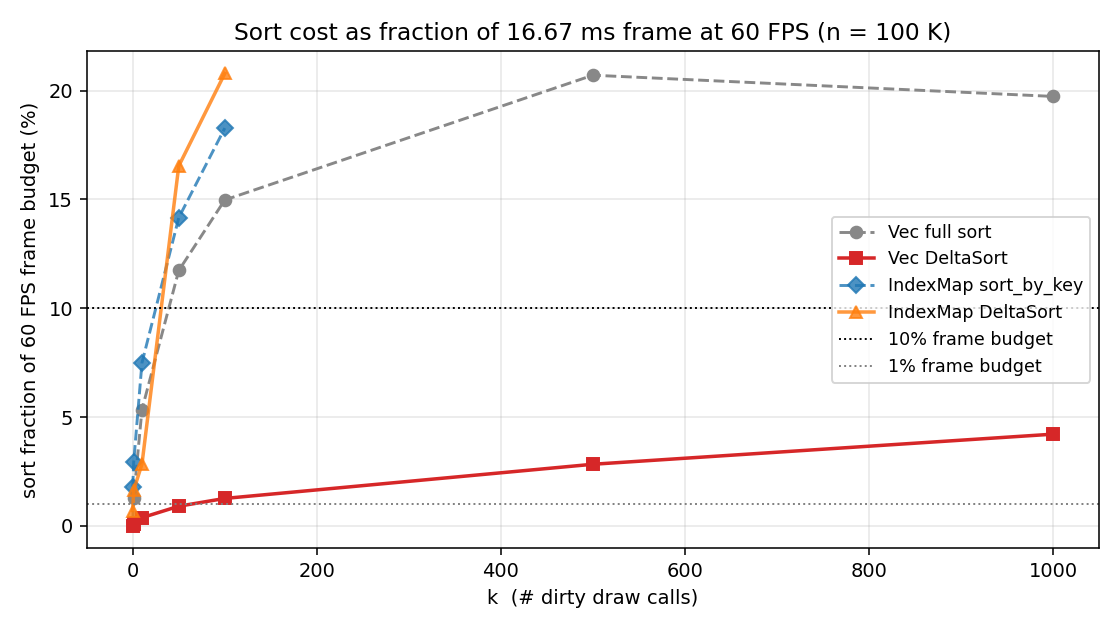
\includegraphics[width=0.7\textwidth]{../figures/track4_bevy_frame_fraction.png}
  \caption{%
    Sort cost as a fraction of the 60\,FPS frame budget.
    All strategies remain below 5\% for realistic $k$.
    The savings from switching to \DeltaSort are invisible in end-to-end FPS.
  }
  \label{fig:bevy-frame}
\end{figure}
